Reminder: Key map (relative for the camera): 
\begin{itemize}
    \item W: forwards
    \item S: backwards 
    \item A: left
    \item D: right
    \item Q: upward
    \item E: downward
    \item U: pan left (yaw)
    \item O: pan right (yaw)
    \item I: pan up (pitch)
    \item K: pan down (pitch)
    \item J: rotate left (roll)
    \item L: rotate right (roll)
\end{itemize}

\section{Task 1: More polygons than you can shake a stick at}
\subsection{c)}
The colourful results are here \cref{fig:task1c}. I ended up moving the camera a bit up as well, so that it was easier to see the whole crater. 

\begin{figure}[tp]
	\centering
	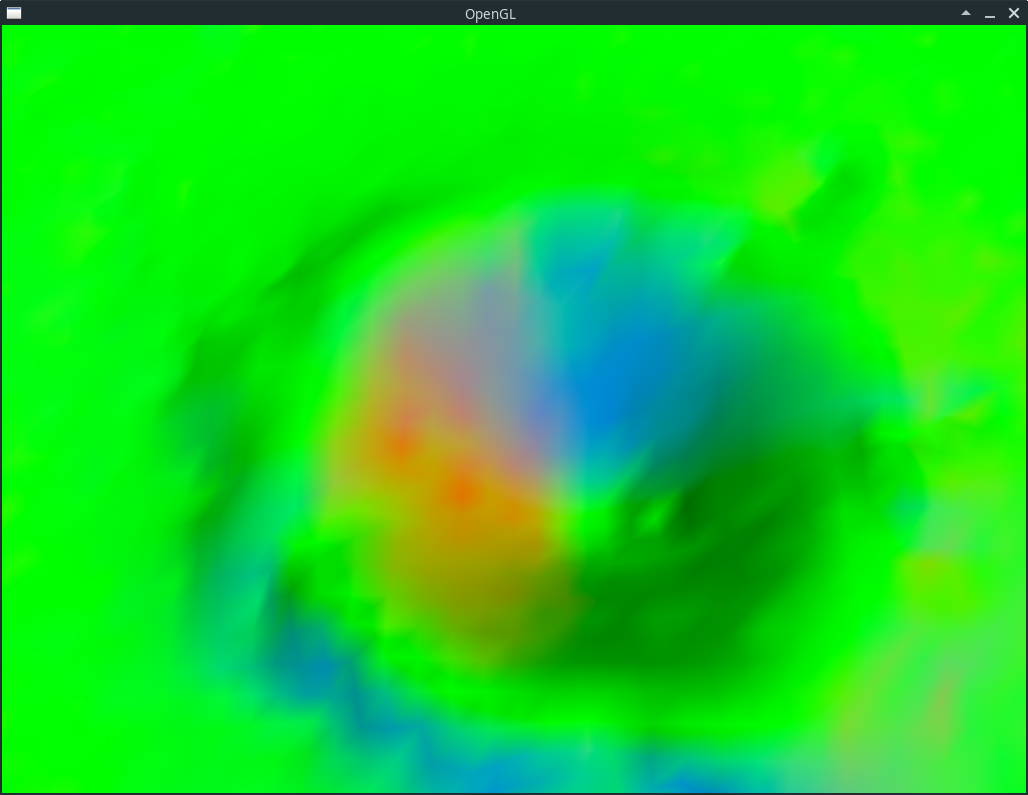
\includegraphics[width=1.00\textwidth]{figures/task1c}
	\caption{Moon landscape with fantastic colours, and camera placed inside a crater}
\label{fig:task1c}
\end{figure}

\newpage
\subsection{d)}
The lit up result can be seen here \cref{fig:task1d}:

\begin{figure}[tp]
	\centering
	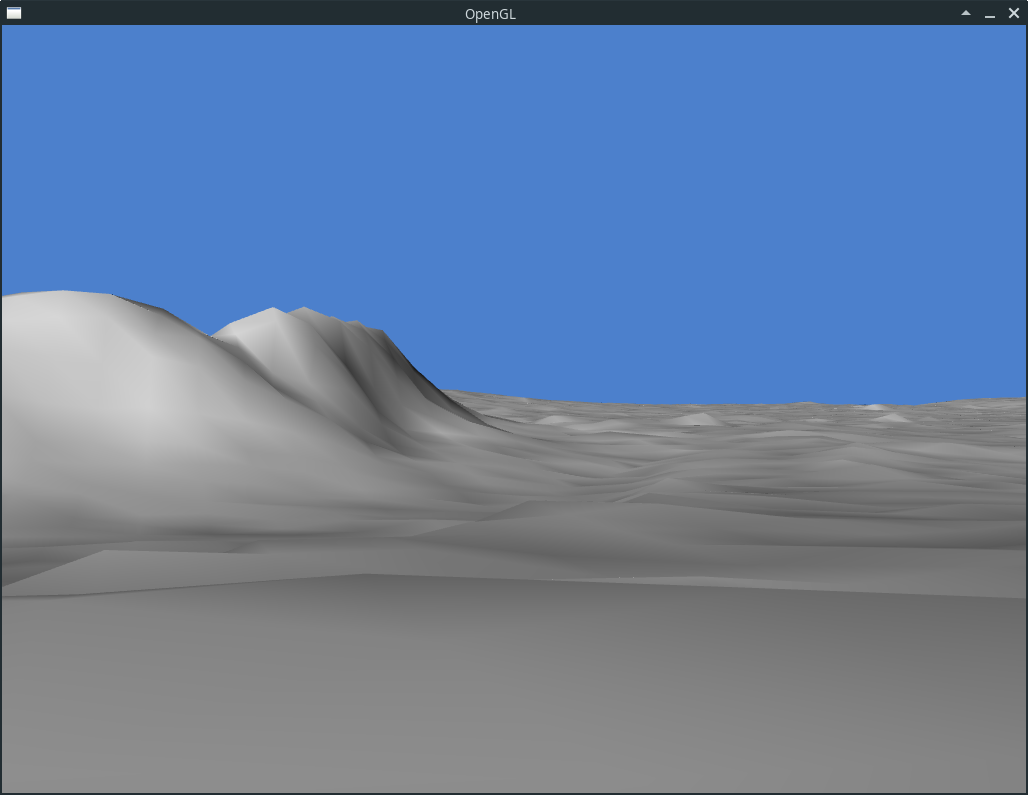
\includegraphics[width=1.00\textwidth]{figures/task1d}
	\caption{Implementation of the Lambertian lighting model}
\label{fig:task1d}
\end{figure}
